\documentclass[journal,10pt,draftclsnofoot,onecolumn,compsoc]{IEEEtran} \usepackage[margin=0.75in]{geometry} 
\usepackage[utf8]{inputenc}
\usepackage{pdflscape}
\usepackage[utf8]{inputenc}
\usepackage{graphicx}
\usepackage{titling}
\graphicspath{ {./Figures/} }

\title{CS Capstone Team 12 - USLI\\Design Document}
\author{Leif Tsang, Donald "Trey" Elkins, Ryan Wallerius}
\date{November 2018, Revised April 2019}

\begin{document}



\begin{titlingpage}

\maketitle
\begin{center}


\includegraphics[scale = 0.25]{Figures/2019patch.png}\\[1.0cm]


\begin{abstract}
The purpose of this document is to explain and enumerate the various systems that the CS team is required to implement for competition in the 2019 NASA University Student Launch Initiative. Covered systems include
the avionics and telemetry unit for rocket flight, the robotic soil-collecting payload, and the team website for front facing documentation and digital presence. This document will cover the functional components and design rationale for each system, and team plans for moving forward with a series of competition-worthy software products.
\end{abstract}
\end{center}
\end{titlingpage}

\newpage
\tableofcontents
\newpage

\section{Revision Table}
Sections have been incremented by 1 from our drafts to our final draft because of the addition of the revision table.
\begin{table}[h]
\centering
\begin{tabular}{|l|l|l|}
\hline
Section & Original & New \\ \hline
3.1 & \begin{tabular}[c]{@{}l@{}}Object detection \\ using computer vision.\end{tabular} & \begin{tabular}[c]{@{}l@{}}Small technical changes\\ to object detection using \\ computer vision that did \\ not get implemented.\end{tabular} \\ \hline
3.2 & State Diagram & \begin{tabular}[c]{@{}l@{}}Changed State Diagram to \\ reflect final structure. Also\\ changed text to reflect these \\ changes.\end{tabular} \\ \hline
3.3 & Class Diagram & \begin{tabular}[c]{@{}l@{}}Changed diagram to show used\\ functions and updated components.\end{tabular} \\ \hline
4.2.1 & N/A & Added a beaglebone black section. \\ \hline
4.4 & N/A & Added a components section. \\ \hline
4.5 & N/A & Added a systems section \\ \hline
5.1.2 & Redux & Removed Redux \\ \hline
5.1.4 & Webpack & Removed Webpack \\ \hline
5.2 & User Use-Case & \begin{tabular}[c]{@{}l@{}}Updated User Use-Case to reflect\\ final structure\end{tabular} \\ \hline
5.3 & Admin Use-Case & \begin{tabular}[c]{@{}l@{}}Updated Admin Use-Case to reflect\\ final structure\end{tabular} \\ \hline
2.4 & N/A & Added GPS \\ \hline
3.1.1-3.2.3 & N/A & \begin{tabular}[c]{@{}l@{}}Removed 433 MHz references, more \\ info on PLEC and talked about new \\ GPS system.\end{tabular} \\ \hline
3.3 & N/A & Removed references to 433 MHz system \\ \hline
3.4 & N/A & \begin{tabular}[c]{@{}l@{}}Modified project objectives to be in line\\ with what we actually worked on.\end{tabular} \\ \hline
\end{tabular}
\end{table}


\section{Introduction}

\sffamily

\subsection{Purpose}
The purpose of this document is to define software systems in order to give the team an overall understanding of the design of each component. This will provide our sub-team and the entirety of the USLI team insight into the topics covered throughout the implementation of the project.

\subsection{Scope}
The avionics, payload, and website will be utilized to compete in a competition hosted by NASA. The mission consists of a single-state solid propulsion rocket being launched to a target altitude of about one mile. At apogee, the rocket separates into 2 sections and safely touches down on the ground using an integrated recovery system. The avionics system tracks the location of the launch vehicle for the duration of the flight. After landing, the aft section of the rocket ejects a robotic payload that must move at least 10 ft. from the rocket body, collect a soil sample with a minimum volume of 10 ml, and then store the sample in a sealed container on-board the payload. Once collected, the sample will be taken to a base station for analysis. The base station analysis is not a part of the NASA competition, but the team decided to pursue it to add scientific value to our entry. Furthermore, the team must develop a robust website to deliver technical documents to NASA and display team information and educational outreach efforts.

\subsection{Context}
The mission will utilize programming languages and software utilities to provide commands and control for the hardware devices - namely micro-controllers such as the Teensy 3.6 - that will comprise the computational systems integrated into the launch vehicle and robotic payload. We will use ReactJS and Material-UI to design and build a website that is capable of delivering technical documents and technical information about the team. The usage of these hardware and software components combined will provide the necessary modules and deliverables for execution of the team's entry for the 2019 NASA Student Launch Initiative Competition.  
\subsection{Glossary}
\begin{itemize}
    \item \textbf{ATU} - Avionics Telemetry Unit: a series of micro-controllers, sensors, and transceivers that collects, transmits, receives, and logs data during rocket flight.
    \item \textbf{CV} - Computer Vision.
    \item \textbf{GPS} - Global Positioning System. One of several worldwide navigation satellite networks used in commercial navigation technologies.
    \item \textbf{NMEA} - National Marine Electronics Association, a standardized format for positional data that is widely used by GPS and other positioning systems.
    \item \textbf{PLEC} - Payload Ejection Controller, receives signal from the ATU ground station to fire off black powder charges and eject the robotic payload from the launch vehicle aft.
    \item \textbf{ReactJS} - A JavaScript library to provide user interfaces through small scripts known as 'components'. Will be used in concert with the Material-UI library. 
    \item \textbf{USLI} - University Student Launch Initiative, a yearly competition hosted by NASA in which university teams compete to build, launch, and operate a rocket and scientific payload. Frequently used to reference the OSU competition team itself.
\end{itemize}

\newpage

\section{Avionics}
The Avionics Telemetry Unit (ATU) is responsible for the generation, logging, filtering, transmission, reception, and output of position and telemetry data while the rocket is in flight. The ATU assists in recovery of the rocket components after launch and collects data which is analyzed via software (MATLAB scripts that are not a part of our capstone project) after the flight to extrapolate critical launch data. The avionics system is composed of a ground station and a pair of flight units that communicate wirelessly using a custom packet system during the flight. The flight units collect and transmit the avionics data to the ground station during the flight. The ground station transmits the received flight data to a USB-connected computer that outputs the data over the Arduino serial monitor. The ground station is also responsible for transmitting an ejection signal to the Payload Ejection System (PLEC) once the rocket has landed and is ready to eject the rover. Modularization and functional decomposition of the code for both systems facilitates ease of development and adaptation.

\subsection{System Design}
The avionics system is composed of a ground station and multiple flight units that are placed within the rocket. Each has its own hardware and software components, and the system as a whole works together to ensure the mission profile is met successfully.

\subsubsection{Flight ATU}
The Flight ATU is composed of a GPS module, Teensy 3.6 ARM micro-controller, XBee Pro S3 900 MHz transceiver, and an antenna which are all embedded and connected on a custom PCB created by USLI electrical engineers. The GPS module receives positional data from various navigation satellite networks which it then transmits to the Teensy as NMEA (National Marine Electronics Association) formatted packets via serial communication. The Teensy writes all of the given NMEA-format packets to the on-board SD card, then uses a C/C++ program to discard all non \$GNRMC-type packets, strips unnecessary information out of the \$GNRMC packets, and packages them into a new packet format which is sent over serial to the XBee Pro transceiver module. The custom packet structure has the following information (and more) added to it:

\begin{itemize}
    \item Custom start delimiter - 0x7E
    \item Least and most significant bits for delimiting at the beginning of the packet
    \item Frame type (TX/RX Request)
    \item Frame ID Number
    \item 64-bit Target Address (currently hard coded)
    \item Reserved bytes
    \item Transmit options
    \item Checksum
\end{itemize}

\subsubsection{Ground Station ATU}
The ground station ATU is very similar to the flight ATU, but boasts a different set of code on the Teensy, a larger antenna, and the capability to connect to a computer via serial (USB). The XBee Pro receives the packets from the flight ATU and sends them via serial to the Teensy. If the Teensy detects a packet in the serial buffer, it loads the packet, unpacks it, determines which ATU (of the 2 flight units) it came from, then pipes the data out over the serial interface with the computer. The ground station also boasts a button and switch which are used as safety controls for the payload ejection control signal; both must be activated simultaneously and the trigger code must be flashed for the signal to broadcast.  \newline

\subsection{Design Rationale}
A majority of the design decisions made for the avionics system stem from decisions made during last year's software and electrical engineers. This year, the goal is to modify the embedded avionics code to be at least 25\% shorter, correctly commented, and functionally decomposed (rather than 2-3 large functions, as it was last year). We also want to fix the code for the PLEC and integrate it more effectively with the ground station, and ensure that the avionics code can be ported to a new custom PCB with a new GPS unit.

\subsubsection{Micro-controller}
The Teensy 3.6 was determined to be the most effective micro-controller for both ATUs due to its speed, size, and ease of programming. The Teensy 3.6 has a clock speed of 180 MHz - more than 11 times faster than the 16 MHz processor on a standard Arduino Uno. This makes the Teensy superior for high speed embedded applications with significant data throughput. The Teensy lacks many of the components that many other consumer micro-controllers are shipped with - ex. non-USB power input, large LEDs, heatsinks, pin headers, etc. - giving it an advantageously small power and spacial profile. Support for serial communication and the ability to write to an on board SD card are also critical functionalities that the Teensy offers. A micro-controller was chosen over a small embedded PC such as a BeagleBone or a Raspberry Pi due to the detrimental effects that software overhead such a system inflicts on the data transmission and receiving process.

\subsubsection{GPS}
The old GPS unit was replaced with a UBlox GPS unit with increased compatibility with global navigation satellite systems. The old GPS chip only interacted with the American GPS network, but the new chip can interact with GLONASS, BeiDou, and Galileo. Hardware differences mandated a change in programming and the serial communication protocol in order to accommodate the new keywords utilized by the NMEA format for satellites that aren't on the American GPS network.

\subsubsection{Transceivers}
The XBee Pro S3 900 MHz transceiver is the current de facto Rx/Tx device in the system due to ease of implementation with pre-existing libraries from the manufacturer, the ability to transmit on the 900 MHz band without a commercial license, and the relative power and range that a 900 MHz transmission band offers. The current 900 MHz system is capable of and tested for reliable packet transmission within a 2 mile line of sight distance at 250 mW of power on a high gain antennae; transmission will be at either 210 mW or 250 mW depending on the other transceiver system's power output to keep our signal emission within a reasonable operational range. The competition rules stipulate a combined outgoing signal power of 250 mW as the cap for operation.\newline

\noindent Unfortunately, the 900 MHz band is prone to interference due to its popularity as a license-free consumer radio frequency. The USLI team experienced technical difficulties last year due to the presence of multiple other higher powered RF transceivers operating on the 900 MHz band at the competition. Since the launch vehicles must be set up and wait for a given duration of time, the 250 mW transmission was easily overpowered and data integrity was significantly impeded.\newline

\noindent To combat the problem of interference on the 900 MHz band, the USLI team would like to put together a very basic functioning proof-of-concept prototype of a 433 MHz radio-frequency communication system. 433 MHz transmission offers relatively high data fidelity, a range encompassing the expected flight and landing distance of the rocket, and its infrequent use due to its restricted band status makes it highly unlikely that any interference would occur from other devices on the same frequency. The hope is that such a system can be expanded upon by subsequent teams in order to overcome the shortcomings of the 900 MHz system. The main drawback to using 433 MHz transmission is the lack of modular and ready to use consumer grade radio frequency devices. The USLI team will not be implementing a full 433 MHz system this year due to shortages of personnel, time, and team resources.

%% Trey

\subsubsection{Programming Languages}
AVR compatible C and C++ are the languages of choice for the Teensy and embedded control code; no other high level languages are easily implemented with the given micro-controllers, and AVR assembly is too difficult to reasonably implement without tackling a steep learning curve that the team doesn't have time to address. Furthermore, C and C++ have their own well fleshed-out standard libraries and are compatible with Arduino and XBee Pro libraries. Some MATLAB is also being used to interact with the data that the avionics system generates, but the scripts are already mostly developed and its operation doesn't fall within the jurisdiction of our capstone project.

\newpage
\subsection{Diagrams}
\vspace{1cm}
\begin{figure}[ht]
    \centering
    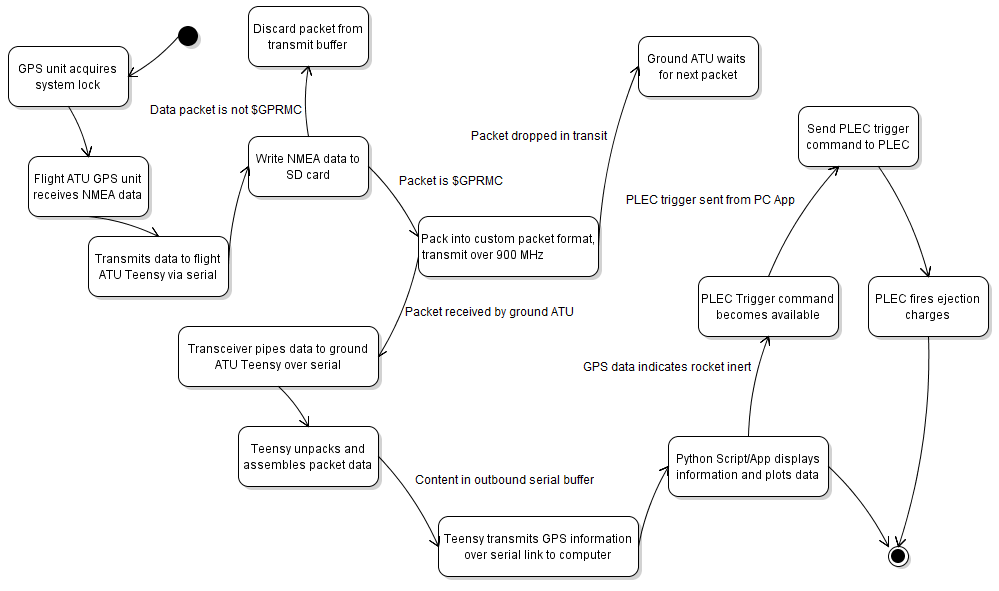
\includegraphics[width = 0.9 \textwidth,angle=0]{avionicsStateDiagram.png}
    \caption{Avionics State Diagram}
    \label{fig:Avionics SD}
\end{figure}

%\vspace{1cm}
\begin{figure}[ht]
    \centering
    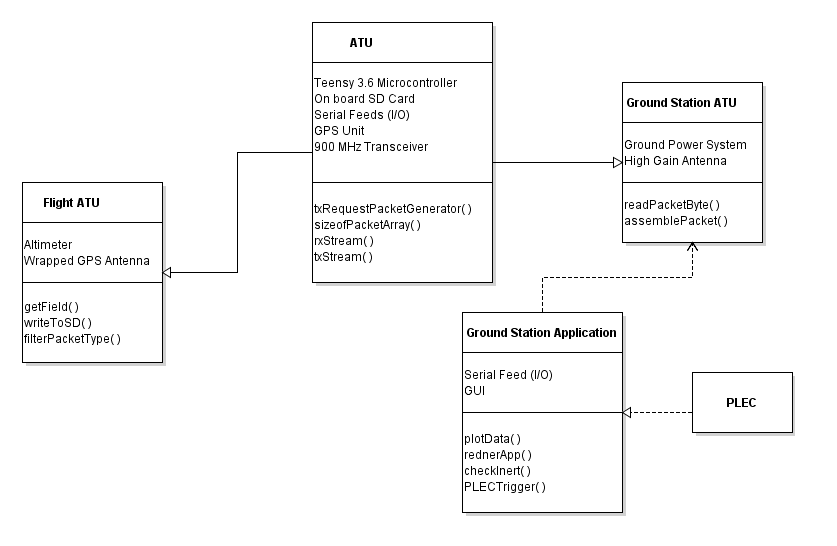
\includegraphics[width = 1 \textwidth,angle=0]{ATUclassDiagram.png}
    \caption{Avionics Class Diagram}
    \label{fig:Avionics CD}
\end{figure}

\newpage
\begin{figure}[ht]
    \centering
    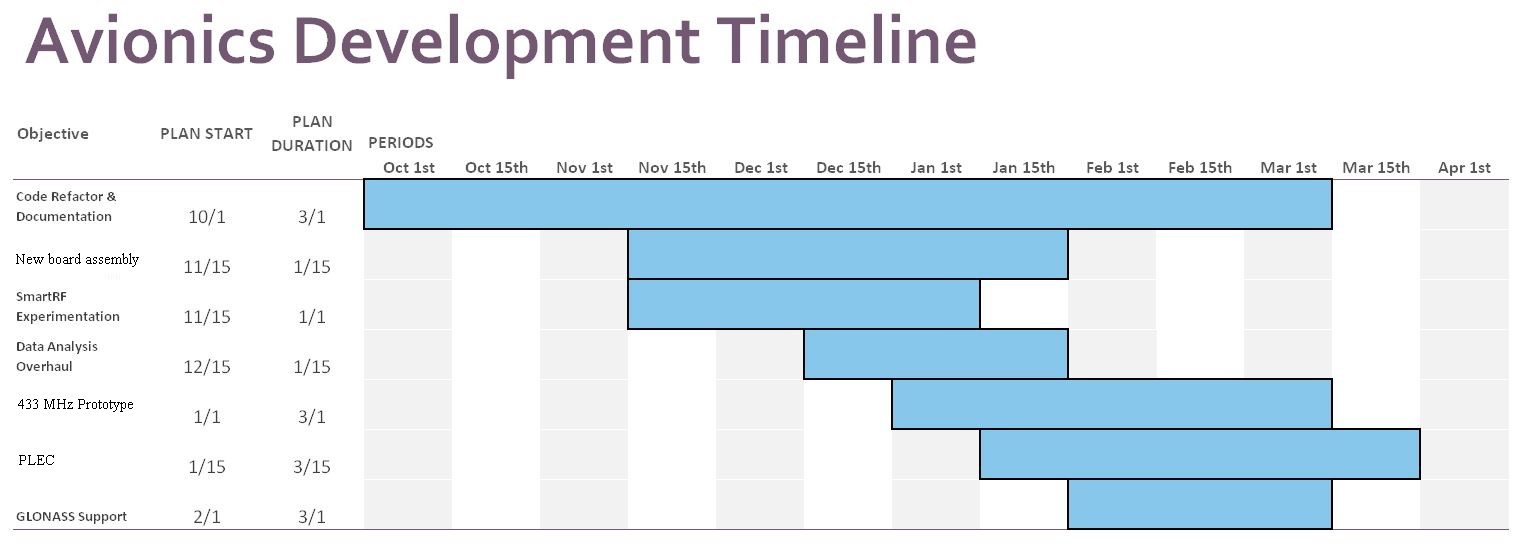
\includegraphics[width = 0.95 \textwidth,angle=0]{ganttATU.JPG}
    \caption{Avionics Gantt Chart}
    \label{fig:Avionics Gantt}
\end{figure}

\newpage
\clearpage

\section{Payload}
The payload will be responsible for a large majority of the mission after ejection. All tasks must be completed while remaining completely autonomous. The tasks that must be completed are the following:

\begin{itemize}
    \item Travel at least 10 meters from any part of the rocket
    \item Find a desirable location to collect a soil sample
    \item Activate auger to collect soil in a sealed container
    \item Receive GPS base station coordinates
    \item Travel to the GPS coordinates sent to the rover
    \item Dock to deliver soil sample that will be released from the rover
    \item Standby to collect and deliver additional samples to the base station
\end{itemize}

\setlength{\parindent}{0cm}
In order to complete the above tasks, the rover must be pre-programmed with a complex set of instructions to follow. The rover will continuously be taking in data from the environment using a camera and sonar sensors to check for obstructions and have the required intelligence to successfully avoid obstacles and remain on track to the destination. The rover is equipped with a GPS in order to guide the robot away from the rocket body to achieve the minimum distance from the rocket body as well as guide the rover to the base station in order to deposit the samples. A gyro will let the rover know if the area being drilled is feasible to obtain a soil sample and if the gyro is within operating range for the auger. The motors must be capable of quickly maneuvering around and over terrain. The rover must have an RF receiver to receive GPS coordinates from the rocket body and the base station for navigation. After the rover obtains the coordinates of the scientific base station, a routing algorithm using GPS and the magnetometer for the heading will guide the rover to the base station for soil sample delivery. 

\subsection{Design Viewpoints}
Practicality was taken into account during the design phase of the rover. The program on the robot will need perform autonomously, so there is no room for error. As such it has been designed with every situation in mind in order to not  become stuck in any specific process. For this reason, there exists an extra computer attached which will be in charge of computer vision. This computer will be responsible for communicating with the Teensy on the rover and giving instructions to follow for docking at the base station. Due to the separation of hardware, the rover would be able to complete the mission even on destruction of non-critical components during ejection (i.e. the BeagleBone - located outside the chassis of the rover). 

\newpage
\begin{landscape}
\subsection{State Diagram}
\vspace{1cm}
\begin{figure}[ht]
    \centering
    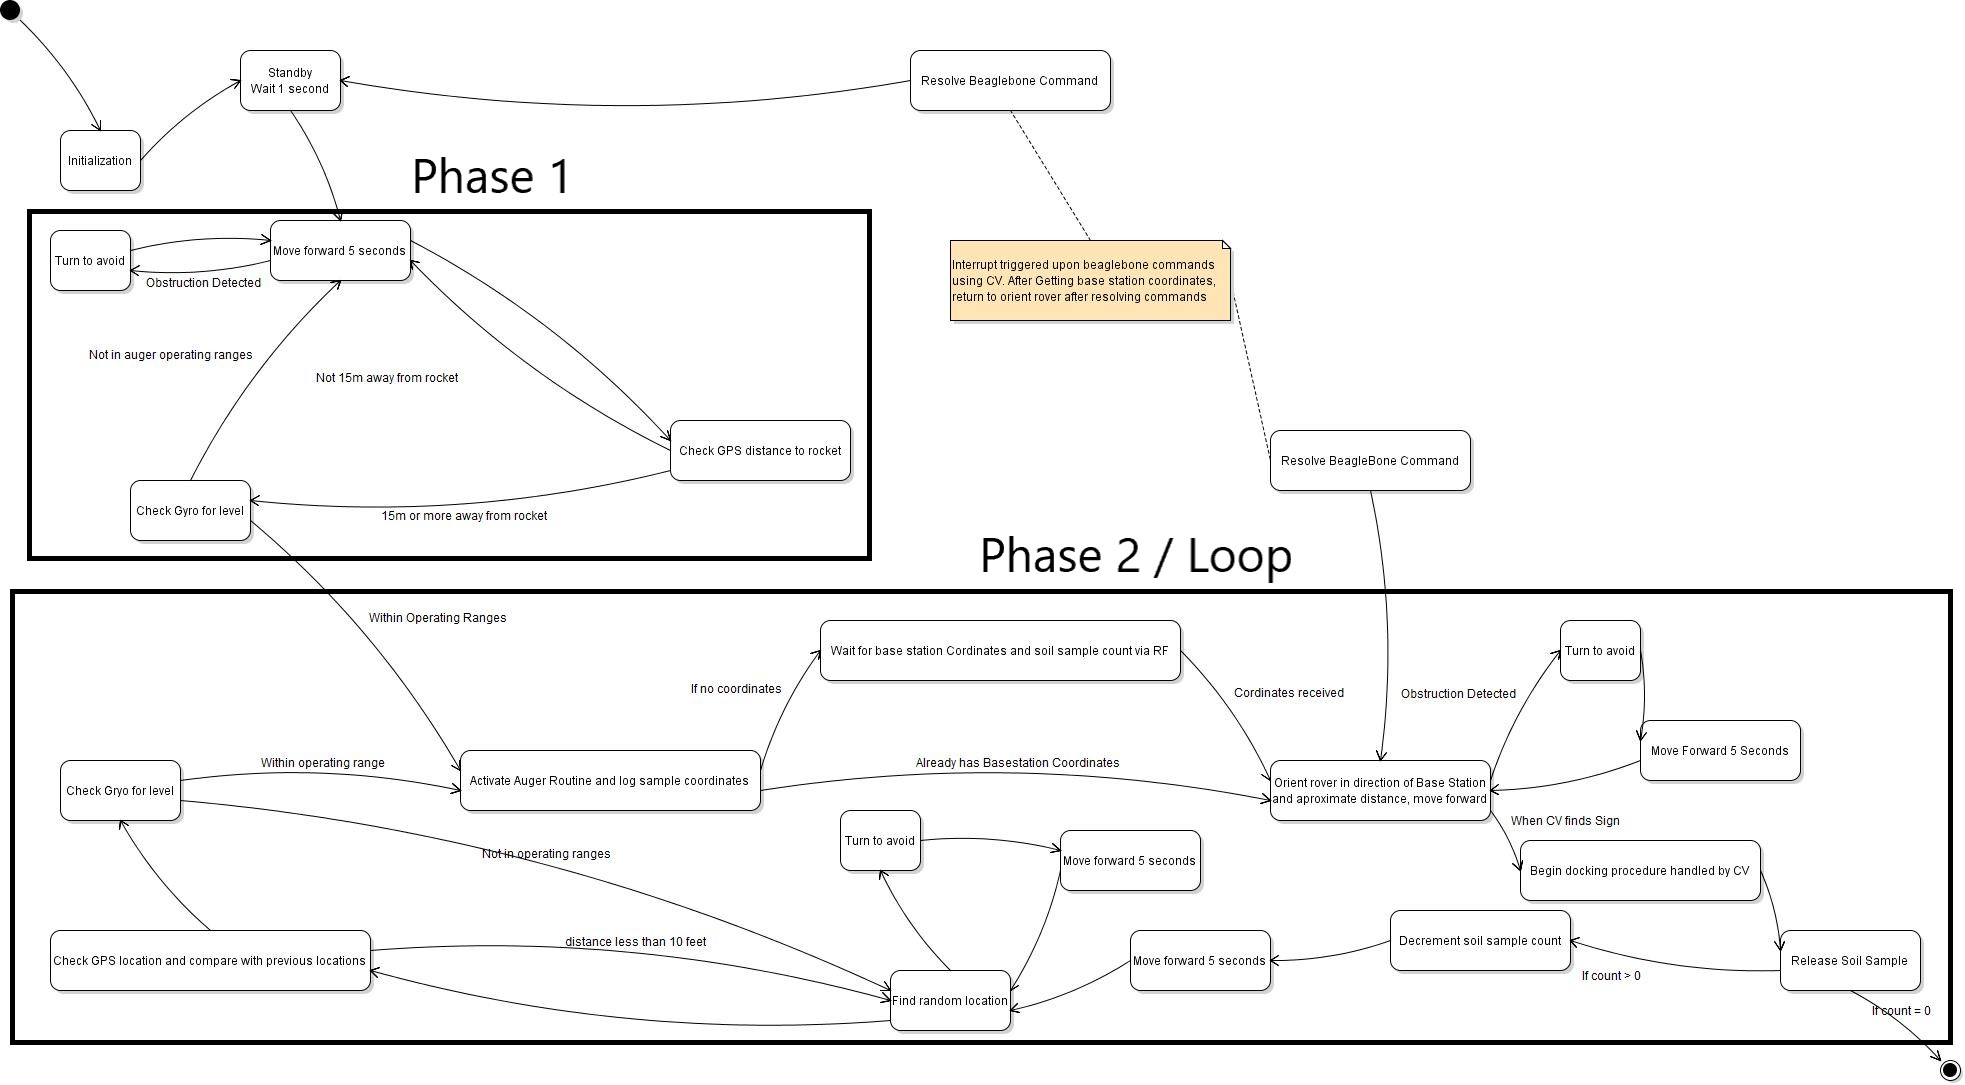
\includegraphics[width = 1.3 \textwidth,angle=0]{Figures/TeensyStateDiag.jpg}
    \caption{Rover State Diagram}
    \label{fig:my_label}
\end{figure}
\end{landscape}

\newpage
The state diagram shown above (figure 1) begins after the payload is ejected from the rocket body. The rover begins by initializing when the rover obtains the GPS coordinates of the rocket. The rover will then start phase 1 of its programming. This involves the rover moving forward until it is at least 10 meters away from the rocket while practicing object avoidance and then finding a level spot to collect a soil sample. The distance between the rocket and the soil sample is verified using GPS. After the soil sample has been collected, the rover freezes and waits for a GPS coordinate that will begin phase 2. During phase 2, the rover will begin to deliver the soil sample to the base station using GPS routing algorithms. The rover will travel in the direction of the base station while continuously avoiding obstacles. After the rover is in close proximity of the base station, it will begin searching for a target on the base station using CV. When the target is found, the rover will be fed instructions by the BeagleBone on how to move in order to climb a ramp for the base station. The BeagleBone is able to find the target and transmit the location to the Teensy effectively. Due to insufficient testing time, fine tuning for docking was not completed. After the rover successfully climbs the ramp and finds its way to a level surface at the top, the rover will check the gyro for level ground and release the soil sample on the level surface. After the sample has been delivered, the extra base station activity will be complete. If extra samples are required the rover will continue on back down the ramp in order to fetch more samples. The number of samples are specified during transmission of the base station location.

\subsubsection{BeagleBone Black}
The BeagleBone is programmed using OpenCV 3 to detect for circles with a Hough Circle transformation after the image grabbed is processed through a grey-scale and canny filter in order to look for hard lines. These lines are fine tuned in a way such that they will not detect false positives. This is done by only allowing edges to be drawn for images with black on white. For this reason a black target on white paper is used. This was to circumvent the possibility of triggering false positives on objects such as tractor wheels that might be on the farmlands of the launch site. The image is then processed and fine tuned to only detect on a strong correlation to a circle that would be found on the target. As a result the BeagleBone was able to consistently detect the target while having very few false positives even in the worst environments. The target was tested to a 45 degree angle while still consistently detecting the target. After the circle is detected, the center point of that circle is then converted into a certain number of pixels left or right of the center of the frame. An instruction for each detected frame is fed to the Teensy over UART in an instruction that looks like "L-1!" or "R-640!". This gives the Teensy measurements to work with to determine the amount to turn in order to climb up the ramp. The Beaglebone is able to run at 0.3 frames per second while a target is recognized or 0.7 frames per second while no target is found. A resolution of 720x1280 was chosen as to get the maximum accuracy and range while not slowing down the frame rate more than necessary. 

\newpage

\vspace{0.5cm}
\subsection{Component Diagram}
\vspace{1cm}
\begin{figure}[ht]
    \centering
    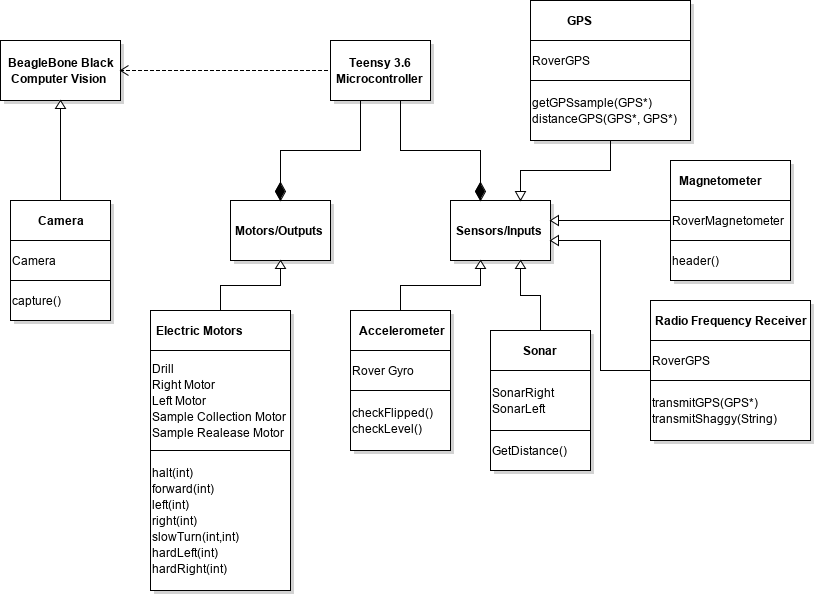
\includegraphics[width = 1 \textwidth,angle=0]{ClassDiag.png}
    \caption{Rover Component Diagram}
    \label{fig:my_label}
\end{figure}
\vspace{1cm}

This class diagram shows the relation of the different components and sensors to the Teensy micro-controller and BeagleBone computer. It shows what hardware will be used and what commands may be used to interact with each device. These devices will be implemented with the functions for controlling each piece of hardware on a lower level. This will help organize the code into a modular arrangement where devices can be called as they are needed for the rover's programming. The BeagleBone is connected to the Teensy as it will be sending interrupts to call specific routines that will be pre-programmed onto the Teensy. Connected to the BeagleBone is a camera that will be able to take a frames to process of the area in front of the rover throughout program.

\subsection{Components}
\subsubsection{Motors}
The motors will be controlled with multiple functions that will set the motors to specific power levels relating to the input that they have been given. The motors use power values between 0 and 255. Each function steadily changes the power by 1 each 10 milliseconds so that the motors do not take any damage and the rover will not tip over from an abrupt stop. Many of the functions are self explanatory: halt will stop the rover, forward gets the rover moving forward. The left and right function cause the rover to move right or left by the movement of 1 wheel while the other wheel is stopped. The hardRight and hardLeft functions however are a little different; These functions cause the rover to turn half the power (given by the parameter) reverse for one wheel and power equal to the value forward for the other. 

\subsubsection{Accelerometer}
This device is used functionally as a gyroscope. When the rover is stopped, the gyro can be read in order to see the direction gravity pulls. The gyro is perpendicular to the ground and thus can be used to find level ground. The accelerometer has two custom functions. checkFlipped will return true if the rover is flipped and checkLevel will return true if the rover is sufficiently close to level.

\subsubsection{Sonar}
These devices are capable of detecting objects in a cone in front of the rover as well as the distance in front of the rover that the object is. A sonar is located on the left and right of the rover which can be used to identify which direction to turn. The getDistance function reads from the sonars giving a value from 0.2 to 5 meters. If no object is located in front of the rover 5 meters is returned. 

\subsubsection{Radio Frequency Receiver/transmitter}
The rover has an XBee antennae on board in order to send transmissions to a partnered antennae which is named Shaggy. This is used to send and receive transmissions from the rover. The main function required for this device is the transmitShaggy function. The project has multiple XBees so the transmission is packetized and de-packetized in order to send the message to a specific XBee, in this case Shaggy.

\subsubsection{Magnetometer}
The magnetometer is responsible for detecting the earths magnetic field. The heading function call works like a compass giving a readout between 0 and 359 in degrees. This is used by the routing algorithms in order to keep the rover traveling the correct direction. The magnetometer is shielded underneath by MuMetals which act to keep the electromagnetic fields from the rover and proto-board from interfering with magnetic field readings. 

\subsubsection{GPS}
The GPS system establishes lock in approximately 2-3 minutes without interference. This is read as a \$GNRMC formatted instruction and parsed with a regex in order to make a GPS object that is used many times throughout the rover mission for calculations and data recording. The distanceGPS function is an algorithm that reads the distance between two GPS objects that are passed in. Another function was also created in order to find the heading required to navigate from one GPS coordinate to another. Two GPS routing algorithms were created. The first of which is to move toward the GPS coordinate by calculating a heading and comparing that value to the value given from the magnetometer. The other is to move away. This reflects the point to move away from over the rover and multiplies that number by 5. This will insure that the rover is always moving away from that point. 

\subsection{Systems}
\subsubsection{Soil Collection}
The soil collection system consists of an auger and a collection chamber with a top door and a bottom door. The auger and collection doors all have encoders in order to precisely measure the number of rotations each motors have taken. This is important because the door needs to open half way and close by reversing the same number of rotations to guarantee that the soil sample is sealed. More importantly the auger has a decoder in order to travel the correct distance while drilling into the earth. If the motors were to spin too far the auger enclosure would be destroyed by the motor. Using a decoder, the number of rotations down can be calculated and the reversed rotations back up can precisely rotate the same number of times back up so any offset can be prevented for the next soil sample. 

The code counts the number of rotations made by the auger and doors using interrupts. For each rotation on the way down, a pin is raised high and a counter is incremented. When that number reaches a specified amount, the counter is reset and can be rotated the opposite direction the same number of times. 

\subsubsection{Object Avoidance}
In order for the object avoidance to be active at all times, the Teensy 3.6 is multi-threaded using a modified teensythreads library. The threading is possible with time division between the main thread and side thread. The main thread is set to run for 100 milliseconds and switch to the "sonar watching" thread for 50 milliseconds. The sonar watching thread is set to watch and trigger an interrupt to itself whenever either one of the sonars detect an object within 0.8 meters. When the teensy is interrupted, a function for avoidance is run and causes the rover to hardRight or hardLeft in the direction indicated by which sonar has been triggered. As soon as the object is no longer detected, control of the rover is passed back to main and the threading will continue. Object avoidance is disabled by suspending the sonar watching thread during times it is not needed and restarted after the task has been complete. 

\newpage
\begin{landscape}
\subsection{Gantt Chart}
\vspace{3cm}
\begin{figure}[ht]
    \centering
    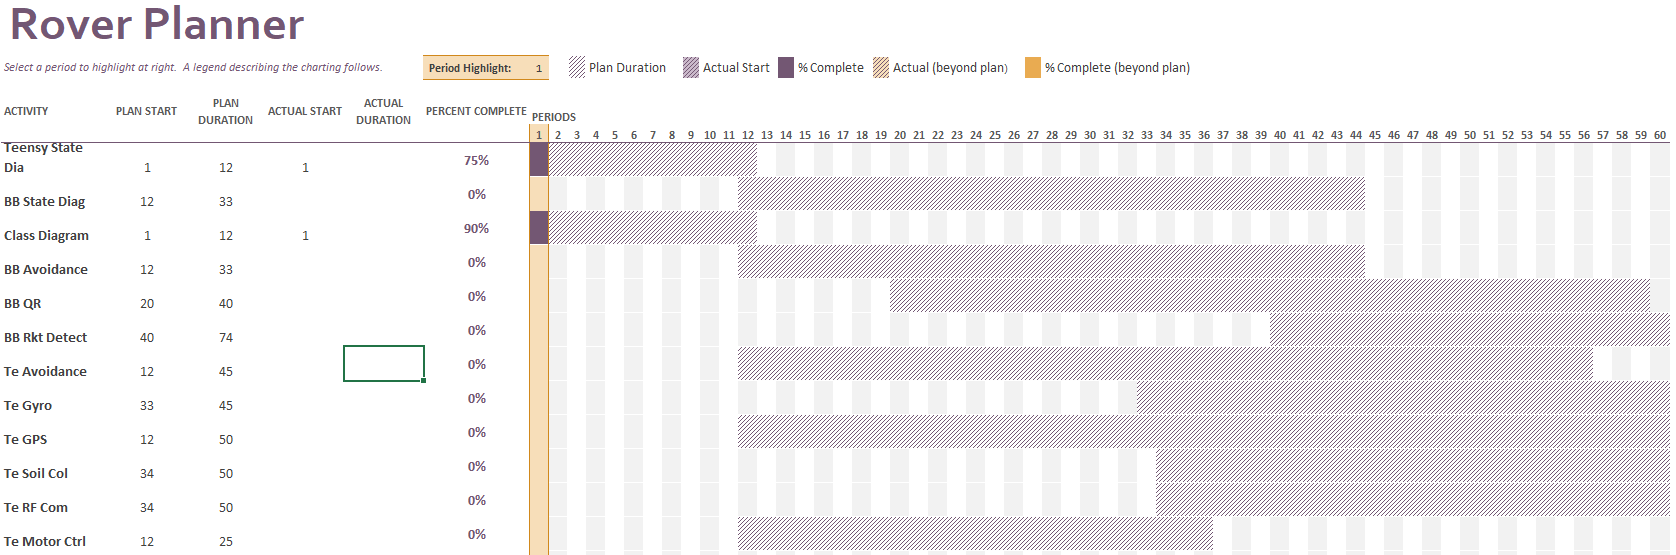
\includegraphics[width = 1.3 \textwidth,angle=0]{PayloadGantz.PNG}
    \caption{Payload Gantt Chart}
    \label{fig:my_label}
\end{figure}
    Each period will account for 1 day and the first period began on November 28, 2018
\end{landscape}

\newpage
\section{Website}
The website is the central location for the storage of critical documents for NASA to retrieve, one of the key social media presences for the OSU USLI team, and a location that sponsors can easily access to learn more about our team. In order for this to be created the the following will be implemented: 
\begin{itemize}
    \item React JS
    \item Redux
    \item Node.JS
    \item Webpack
    \item Browser Sync
    \item Babel
    \item Material-UI
\end{itemize}
Although the website is not directly a part of the competition, creating a website is crucial to the team's success. The website will be aesthetically pleasing, easy to navigate, and easy to access. React is also used because of the versatility with regards to mobile development.  

\subsection{Technologies Implemented}
\subsubsection{ReactJS}
ReactJS is an open-source JavaScript used to build user interfaces specifically for single page applications. The purpose for development was to handle the viewer layer for web and mobile applications. React allows developers to create large web applications which can change data and interfaces without reloading the page. React is also fast and simple. This allows our development team have the tools it needs in order to meet the goals set by the USLI team. 
\subsubsection{Node.JS}
Node.js is a an open-source environment that executes JavaScript code outside of a browser. Developers use Node.js for client-side scripting. Node.js allows developers to run scripts server-side to produce web page content before the page is sent to the user's web browser. Our team is using Node.js on our website so we can run multiple tasks simultaneously. This also meets the team's goal of efficiency. 
\subsubsection{Browser Sync}
Browser Sync will be a crucial tool that the team uses for testing. Browser Sync makes changes and testing faster by synchronizing file changes and interactions across many devices. This feature is called Live Reloading and makes the page auto-reload when changes in code are made. This is implemented in the background and will help our team coordinate multiple developers while accessing and developing the new website.  
\subsubsection{Babel}
Babel is a JavaScript compiler that has the following features: 
\begin{itemize}
    \item Transform syntax
    \item Polyfill features missing in target environment
    \item Source code transformations
\end{itemize}
This is also done in the backend and helps with development. 

\subsubsection{Material-UI}
Material-UI is one of the most used user interface libraries for React. Material-UI has React components that implement Google's Material Design. The following reasons are why we are using Material-UI: 
\begin{itemize}
    \item Deliver on fully encapsulated React components
    \item Customization
    \item Cross browser compatibility and accessibility
    \item Ease of learning
\end{itemize}
Material UI was used to help create the Home page, About Us section and the Deliverables. Templates and examples were given as well as support. 
All of these tools will give the team the ability to develop a website that will meet the goals set and contribute to the team's success. 

\newpage
\subsection{User Use-Case Chart}
\begin{figure}[!htp]
    \centering
    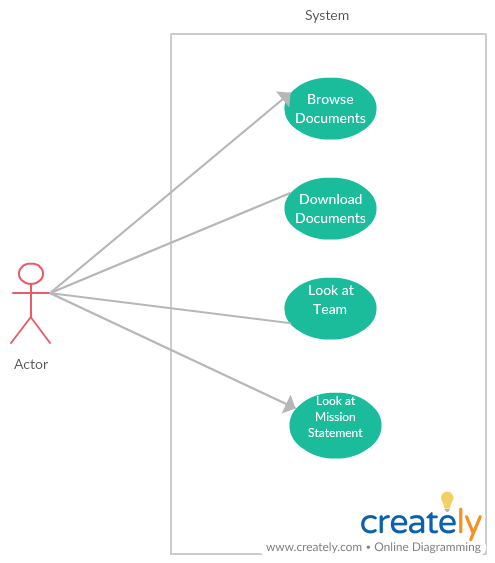
\includegraphics[scale = 0.5, width = 1 \textwidth,angle=0]{Website_User_Use_Case.png}
    \caption{Use Case - User}
    \label{fig:my_label}
\end{figure}
This figure shows what the user is able to do when they access our website. We will have an About Us section, Documents section and Home page. NASA needs to be able to download our documents that we submit for the competition so there will also be an option to download the pdfs. 

\subsection{Admin Use-Case Chart}
\begin{figure}[!htp]
    \centering
    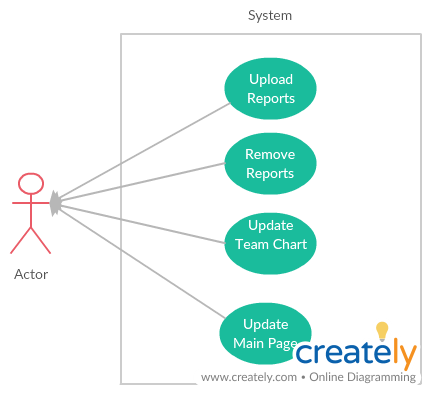
\includegraphics[width = 1 \textwidth,angle=0]{Figures/Admin_User_Use_Case.png}
    \caption{Use Case - Admin}
    \label{fig:my_label}
\end{figure}
This figure shows the options that the admin of the website has. We will have pictures of the team up so they will be able to update the website with current pictures. Admins can also update our progress, add documentation needed for NASA and update the sponsor list. 

\newpage
\subsection{Gantt Chart}
\begin{figure}[!htp]
    \centering
    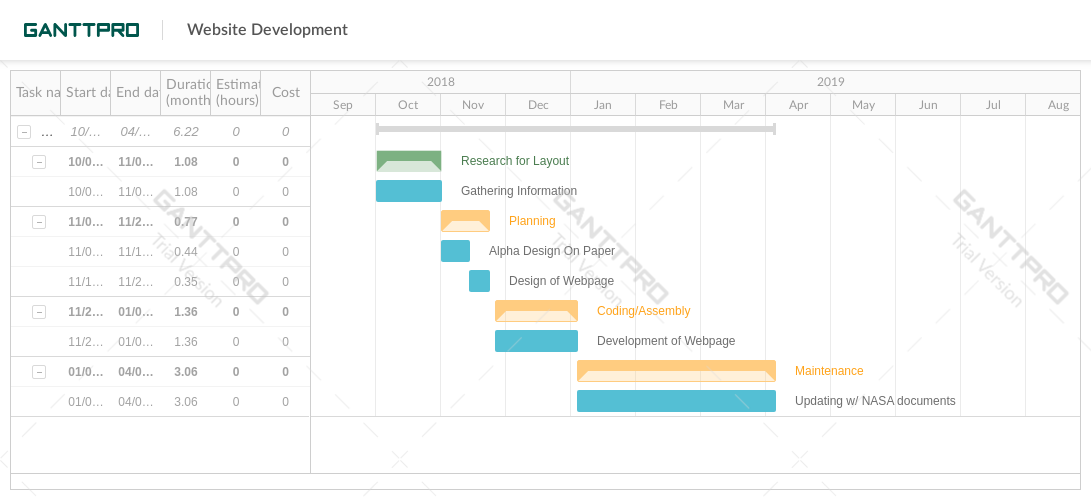
\includegraphics[width = 1 \textwidth,angle=0]{WebsiteDevelopment.png}
    \caption{Website Gantt Chart}
    \label{fig:my_label}
\end{figure}
This figure is an overview of the development of our website for the Oregon State USLI team. We must have a functional product by January 4th. This is when a critical document for NASA is due. After January 4th we will be continuing our development as well as maintenance of the website.  

\newpage
\section{Conclusion}
This document explains and summarizes the avionics, payload, and website systems that the CS team is implementing for NASA's 2019 University Student Launch Initiative Competition. Key terms are explained, design components for each system are enumerated, and design rationale is laid out and expanded upon. The team must apportion the work appropriately, communicate effectively, and work together to deliver the required functional products for OSU's rocket launch at the NASA USLI competition in April 2019. Each system presents its own challenges and obstacles, but each system is critical to OSU's competition entry and potential victory. Care must be taken to ensure that each system is completed to requirements and expectations, and that the best products that team 12 can create are delivered to the USLI team.

\end{document}
